\chapter{Application on Election Data} %of Benford's Law 


We have decided to analyse presidential election results from three countries to showcase how BL can be used for indicative measures. First, we start with the one that we are the most familiar with, the Czech elections in 2023. Up next, the last USA elections. And to finish, the Belarusian elections in 2020, since the data from the last elections was not available. 

In each country, the election system is a little different. In the USA, each state performs its election process according to the state law, and then the results for the entire country are summed up. And the votes do not go directly to the one candidate, but to the electoral college that ends up voting for the candidate. \cite{electoral-college}

This, however, does not affect the performance of the BL analysis due to the scale invariance principle and because no matter the rules, the selection of the votes is still a fraction of the population, so we should be able to get reliable results. 



\section{Presidential elections in Czechia in 2023}

In Czechia, the presidential elections have two rounds. In this analysis we shall focus on the second round. This data was easily accessible through the CZSO website even for individual cities in Czechia. So, the vote counts per city were analysed, since this ensured the largest possible range in data. In the dataset, there are the vote counts from 6254 cities, towns etc. and the foreign votes were manually added. 

\begin{figure}[h]
    \centering
    \caption{The results of the presidential elections on the city level in Czechia in 2023}
    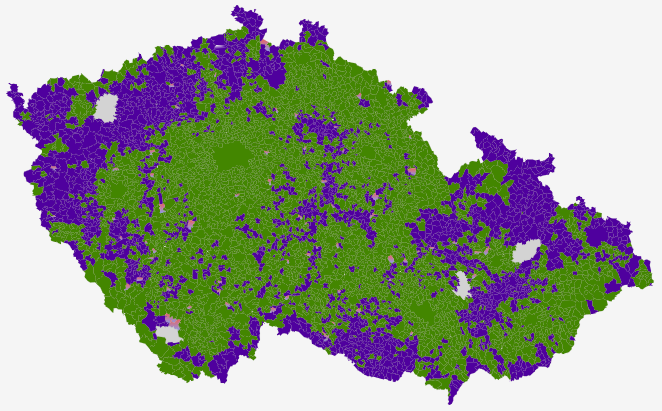
\includegraphics[width=0.7\linewidth]{BT-DT-eng/TemplateBT-DT/img/cz-election-result.png}
    \label{fig:cz-election-result}
    \source{: \citeauthor{CR23data}, \citeyear{CR23data}}
\end{figure}

The final vote distribution on the city-level can be seen on the map in Figure \ref{fig:cz-election-result}. There were two candidates, Petr Pavel (signified by green) and Andrej Babiš (signified by dark violet), pink territory is where the vote share was equal, grey is a territory without a ward. Petr Pavel won with 3,359,301 votes, which is around 58,32\% of all votes. Andrej Babiš got just a little less, 2,399,898 votes, 41,67\%. Turnout was 70,25\% of eligible voters. 99,51\% the votes were valid. \cite{CR23data}

For the totals, both the OOM and OMV were rejected. However, for the individual candidates, the OOM was just a little above 3 when removing the 95. percentile. For this reason, the focus is on the individual candidate counts, rather than on the totals. 


\subsubsection{Relative frequencies of the digits on a given position}

\begin{figure}[h]
    \centering
    \caption{First digit distribution of all votes, Czechia 2023}
    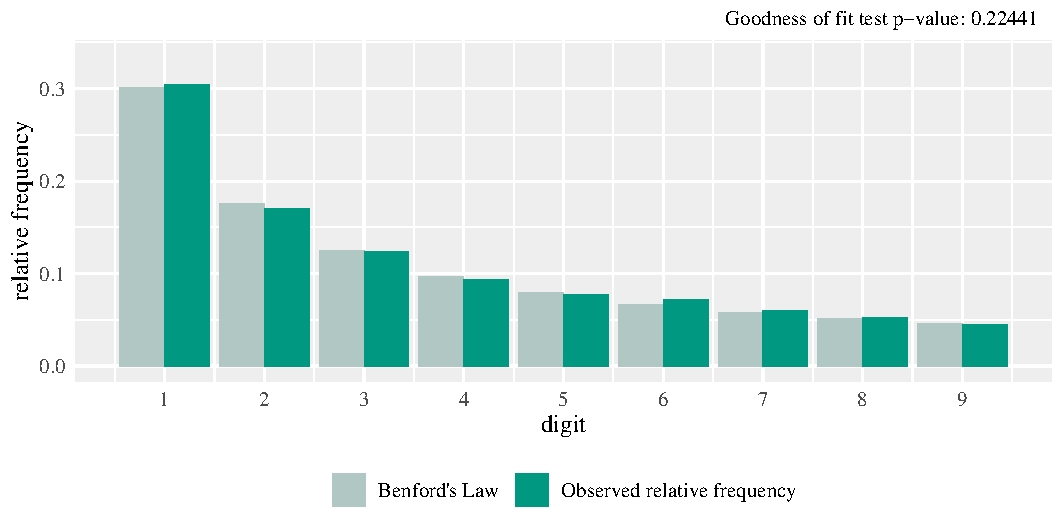
\includegraphics[width=0.99\linewidth]{BT-DT-eng/fig/CZ23-both-first_digits.pdf}
    \label{fig:CZ23-both-first_digits}
\end{figure}

 
\begin{figure}[h]
    \centering
    \caption{First digit distributions of both candidates in Czechia in 2023}
    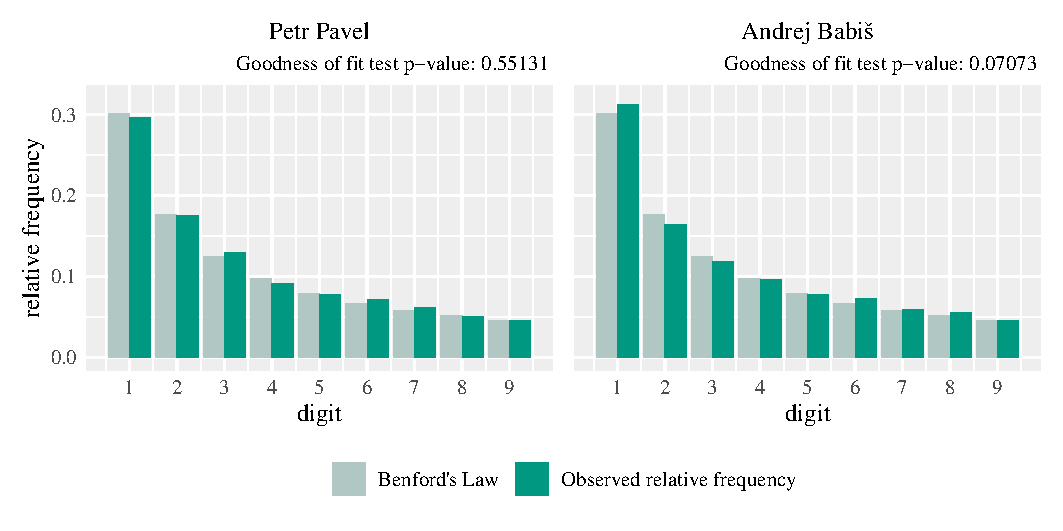
\includegraphics[width=0.99\linewidth]{BT-DT-eng/fig/CZ23-dual-first_digits.pdf}
    \label{fig:CZ23-dual-first_digits}
\end{figure}

In figures \ref{fig:CZ23-both-first_digits} and \ref{fig:CZ23-dual-first_digits} we can see how the data complies very well to the BL first digit law - for all votes as well as for each candidate. In grater detail, the first law compliance can be seen for the first two digits on figures \ref{fig:CZ23-both-first_two_digits} and \ref{fig:CZ23-dual-first_two_digits} in the first appendix. The goodness of fit tests support this by not rejecting their null hypothesis that the relative frequencies are equal. 

\begin{figure}[h]
    \centering
    \caption{Last digit distributions from both candidates in Czechia in 2023}
    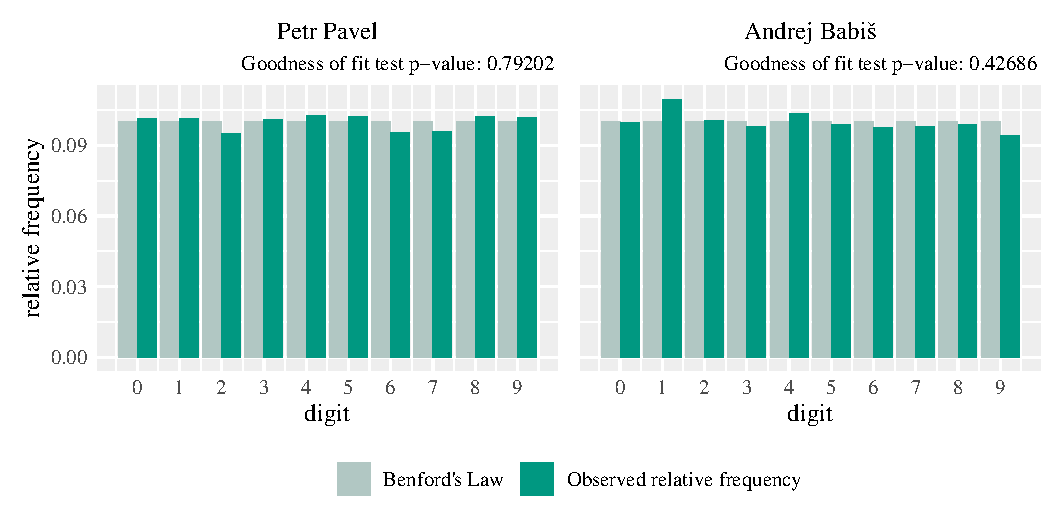
\includegraphics[width=0.99\linewidth]{BT-DT-eng/fig/CZ23-dual-last_digits.pdf}
    \label{fig:CZ23-dual-last_digits}
\end{figure}

 

Then, in figure \ref{fig:CZ23-dual-last_digits} we can see the compliance with the BL last digit law. The goodness of fit test does not reject the null hypothesis that the relative frequencies are close to equal. 

And lastly, the test for the second leading digits compliance is not rejected for either of the candidates as can be seen in figure \ref{fig:CZ23-dual-second_digits}. 

\begin{figure}[h]
    \centering
    \caption{Second digit distributions from both candidates in Czechia in 2023}
    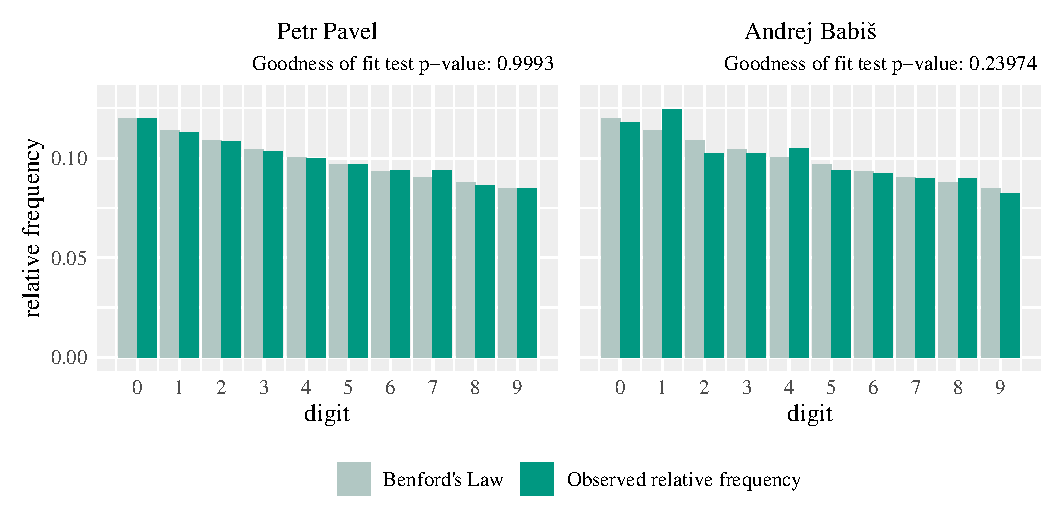
\includegraphics[width=0.99\linewidth]{BT-DT-eng/fig/CZ23-dual-second_digits.pdf}
    \label{fig:CZ23-dual-second_digits}
\end{figure}

Overall, just based on the relative frequencies of the digits on a given position, we can assume the data is genuine and does not contain digital fraud (does not mean there is no fraud of any other origin). Additional evidence can be seen in the first appendix, that contain the distributions of digits on a given position for the total votes (figures \ref{fig:CZ23-both-second_digits} \ref{fig:CZ23-both-third_digits} and \ref{fig:CZ23-both-last_digits}) all of which do not reject the null hypothesis. And for both candidates, there is the plotted compliance of the third digit distribution \ref{fig:CZ23-dual-third_digits}, again not providing any evidence of fraud. 

\subsubsection{Digital development pattern analysis}

For more comprehensive analysis, we can deepen the analysis by observing the digital development pattern in figure \ref{fig:CZ23-digital_development_pattern}. Firstly, we can see that for the smallest integral orders of ten, which are represented by only 0.34\% in the whole dataset, the higher they are the more frequent they are. This aligns with what was expected, as \citeauthor{kossovsky2014benford} mentioned (paraphrased in  \ref{DDPattern} section). When going to the higher orders, the pattern inverts. In the most prevalent interval in the data (middle plot, 52.73\%), the data is close to the BL first digit law. From there, the first digits are more and more frequent, as expected. 

\begin{figure}[h]
    \centering
    \caption{Digital development pattern - Czechia 2023}
    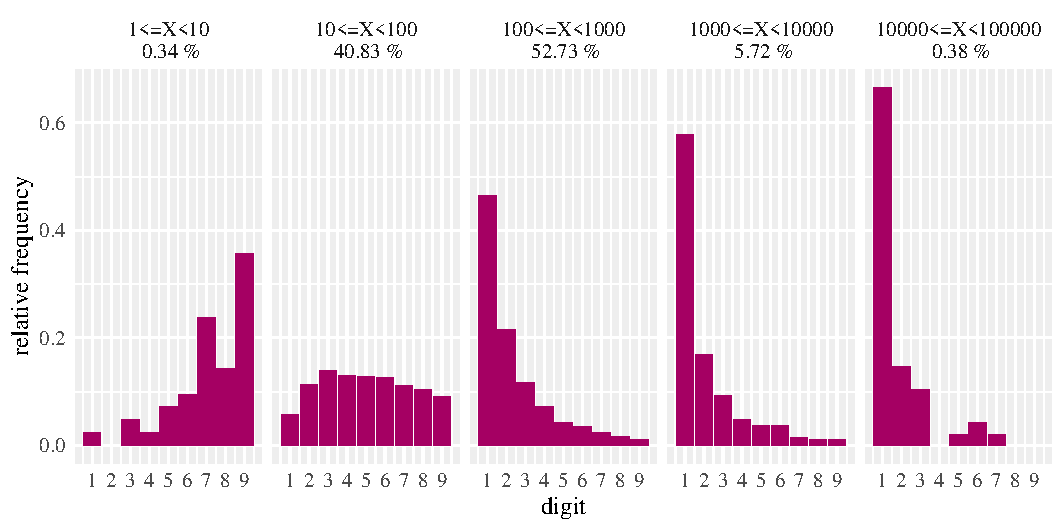
\includegraphics[width=0.99\linewidth]{BT-DT-eng/fig/CZ23-digital_development_pattern.pdf}
    \label{fig:CZ23-digital_development_pattern}
\end{figure}

To conclude this part, the observed digital development pattern aligns with the expected pattern.  


% \subsection{Results}

% In all the tests we have performed, we have not gained enough evidence to reject all of our hypotheses on the compliance of digits to the BL. We can assume that the Czech presidential elections in 2023 are free of any digital fraud. 

% \begin{koment}
%     Doplnit OBSE posudek + ten Lebeda moment 
% \end{koment}

% \begin{koment}
% VERBATIM, PŘEPSAT:

% V České republice se opakovaně setkáváme s poukazy na nejrůznější vady volebního procesu. Běžně se můžeme dočíst o kupčení s hlasy, o podezřele vysokých počtech zneplatněných hlasů, hromadných účelových změnách trvalého bydliště před konáním komunálních voleb, účelovém svážení občanů k volebním místnostem , nedostatečné kontrole hlasovacích místností zejména v noci z pátka na
% sobotu, nekvalitní práci volebních komisí apod. \cite{Lebeda2021}

% Reakce ze strany státu na tyto podněty však byla dlouhou dobu spíše vlažná. Opatření, která by tyto nedostatky eliminovala, byla v minulosti přijímána dosti pomalu. Transparentnosti bychom přitom měli věnovat velkou pozornost, protože spolu s důslednější kontrolou voleb totiž mohou vést k vyšší důvěře v demokratický režim, k vyšší volební účasti a tím pádem i k vyšší
% legitimitě volených orgánů. \cite{Lebeda2021}

% Podezřelé: 
% Rozdíl mezi vydanými a odevzdanými obálkami, podíl neplatných hlasů (špatně odevzdané hlasy), 100 \% využitých preferenčních hlasů (celostátní průměr je asi 12 \%), 100 \% účast... Toto často vede na špatnou práci volební komise. \cite{Lebeda2021}

% Dalším problémem je to, že se volební komise málo obměňují, tudíž k těmto chybám může docházet opakovaně a systematicky. \cite{Lebeda2021}

% \end{koment}


\newpage

\section{Presidential election in the USA in 2024} 

The USA does not have a central statistical service that would provide the nationwide data on a county level, which we need for this analysis. However, \citeauthor{tony_mcgovern_2025_14223604} was able to scrape data from the Fox News website, which provided us with the vote counts for each county as needed. In this dataset 

%This does not add much to the transparency of the election result, but for citizens who do not trust the centralised system, this may seem more transparent, as the results are analysed in the place of election and then ... \url{https://www.usa.gov/electoral-college}, \url{https://bensguide.gpo.gov/election-of-the-president-vice-president-general-election}. 





% \url{https://github.com/nytimes/presidential-precinct-map-2024?tab=readme-ov-file}

% \url{https://github.com/tonmcg/US_County_Level_Election_Results_08-24}

% \cite{tony_mcgovern_2025_14223604}

% \url{https://www.osce.org/files/f/documents/d/e/588772.pdf} - zavery od OSCE, pokud budu chtit vic \url{https://www.osce.org/odihr/elections/usa/572581}

% \begin{koment}
%     jedno velke WTF, ale asi jsem nasla data - scrapnout vsechny tyto webove stranky: https://www.fec.gov/introduction-campaign-finance/how-to-research-public-records/state-election-offices/

%     a budu mit county level data, jenze ted je otazka, jestli mi to za to stoji (odhaduju tak 10 hodin prace) plus jeste teda jde o to, ze kazdy stat to ma trochu jinak a proto tyto votes vlastne asi nedavaji smysl? nevim nevim, moc se mi to nelibi, 
% \end{koment}


\begin{figure}[h]
    \centering
    \caption{The results of the presidential election in the USA in 2024}
    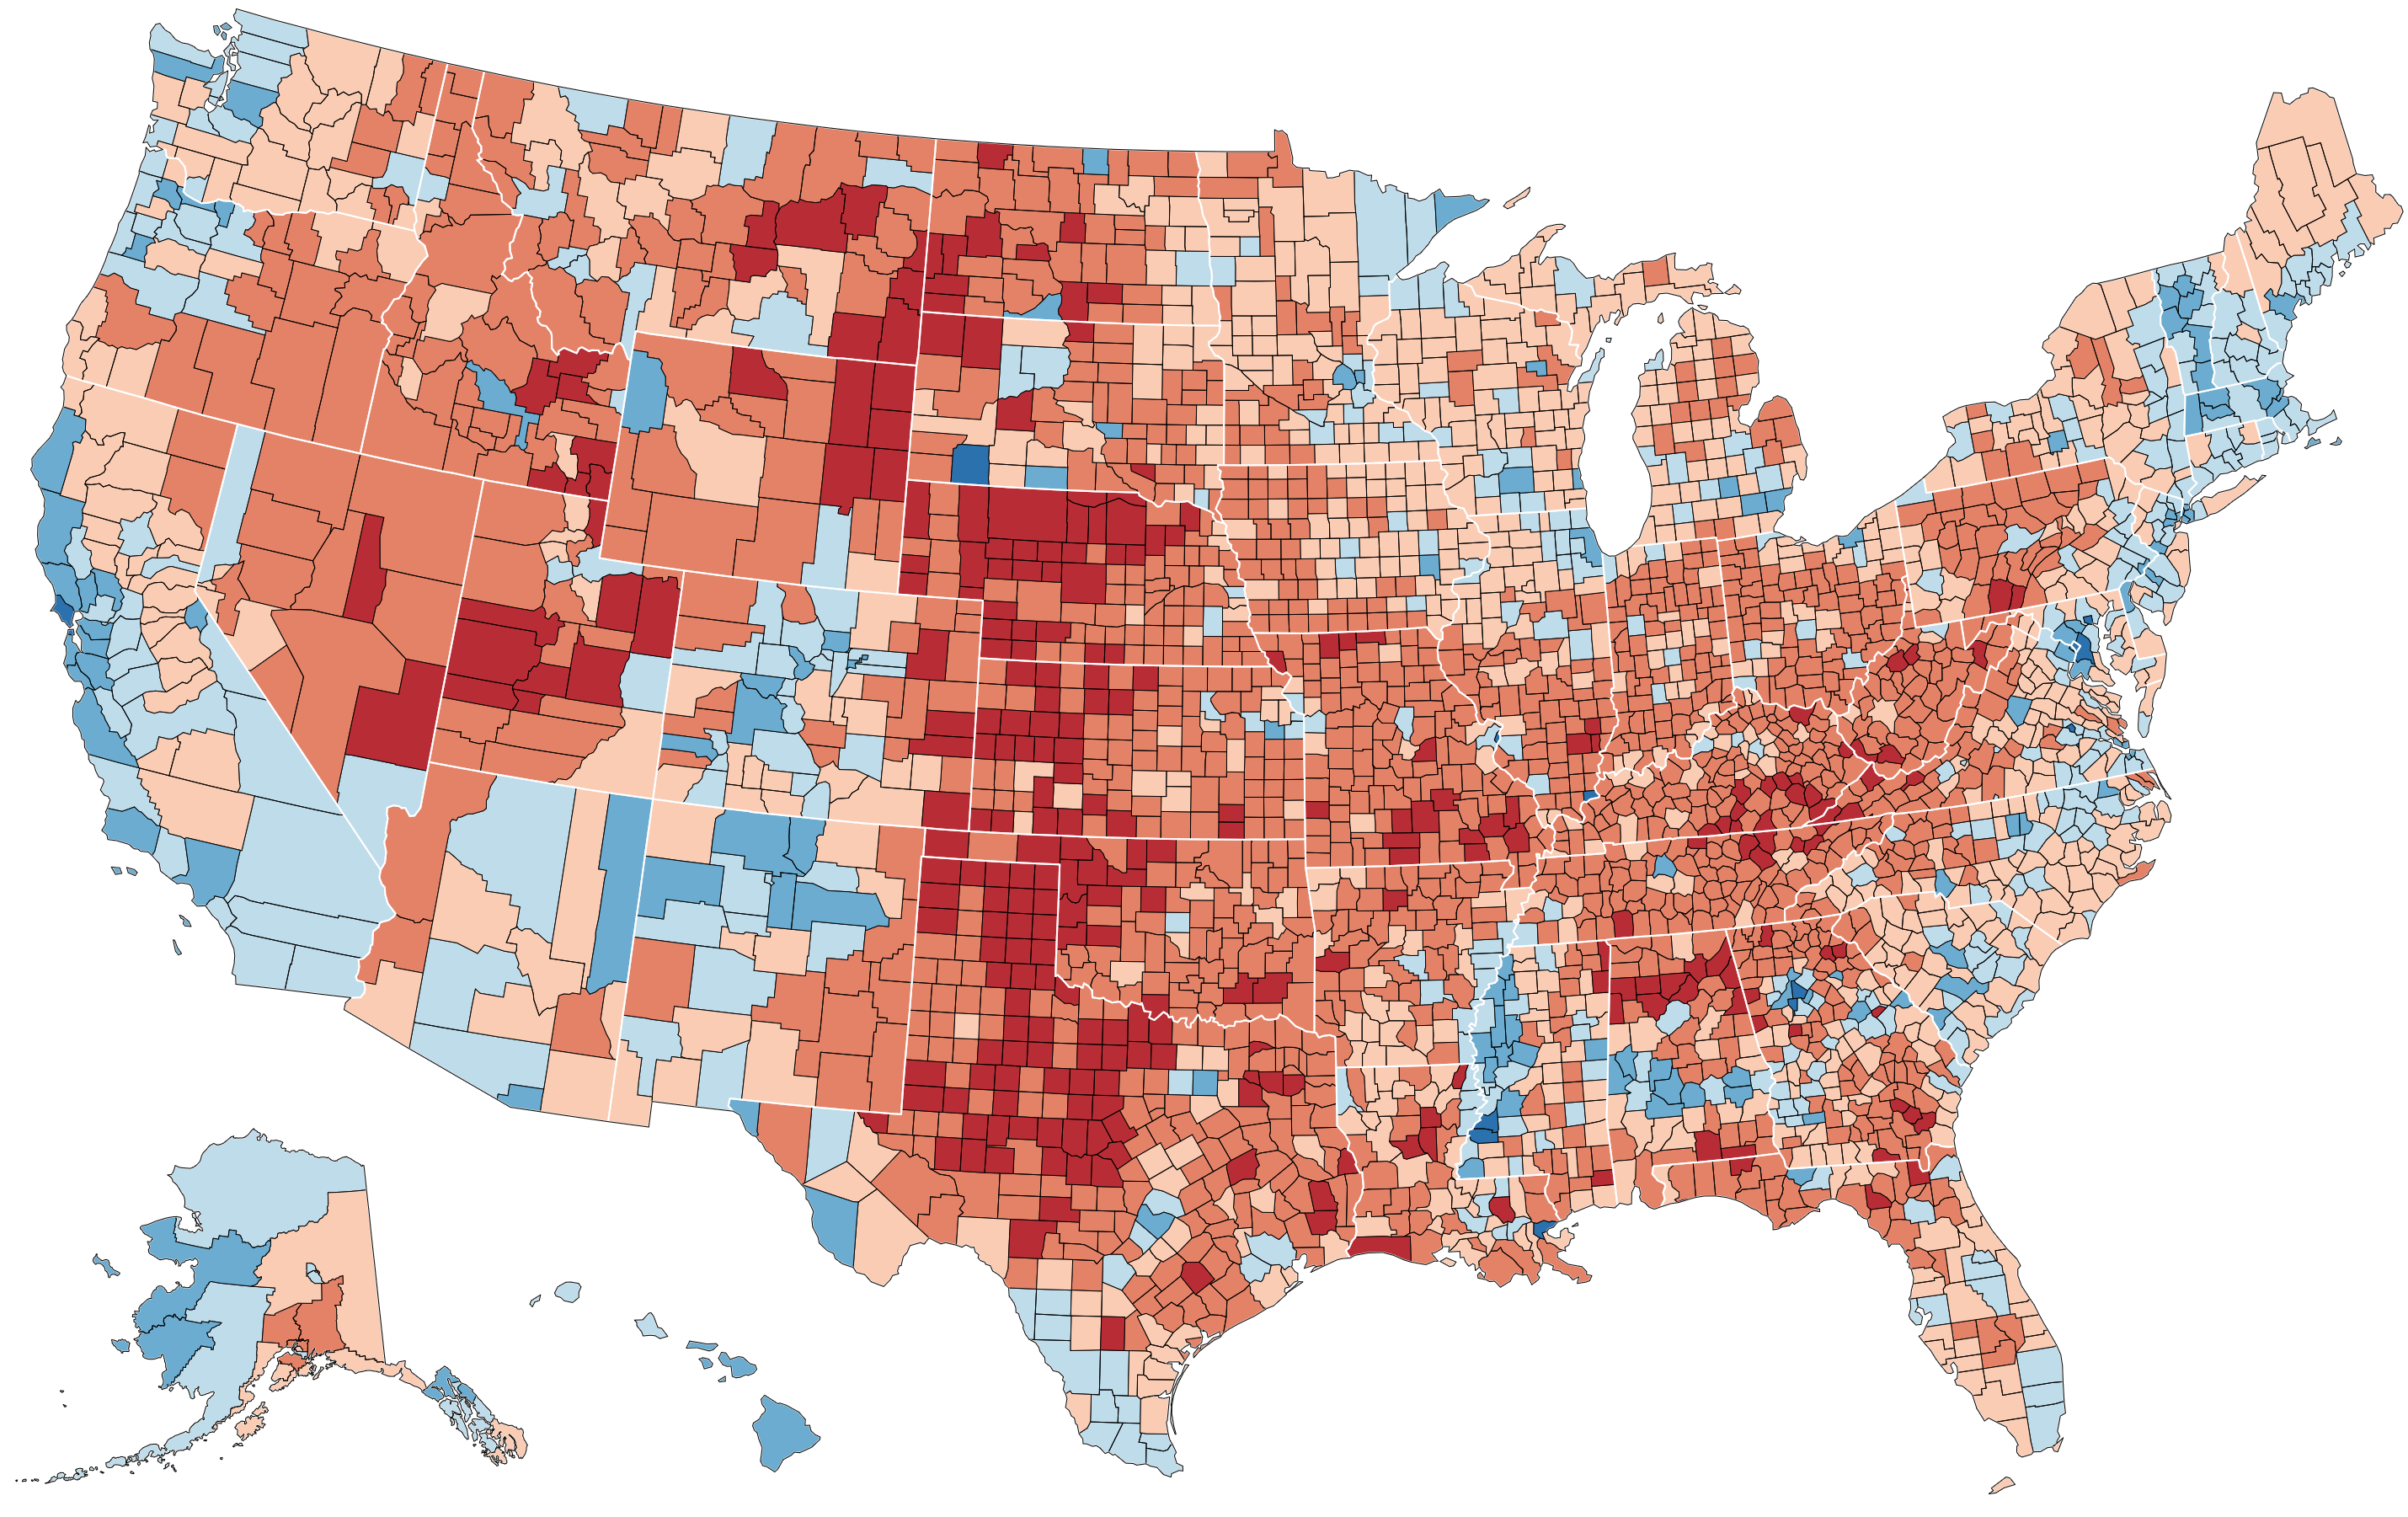
\includegraphics[width=0.75\linewidth]{BT-DT-eng/TemplateBT-DT/img/us_election_results.png}
    \label{fig:USA24-results}
    \source{:  \citeauthor{tony_mcgovern_2025_14223604}, \citeyear{tony_mcgovern_2025_14223604}}
\end{figure}

The election was held on November 5, 2024. Donald Trump won the election with 77,302,580 votes, which corresponds to 49.8\% of the votes. His main opponent, Kamala Harris, acquired 75,017,613 votes in total, which is about 48.3\%. The rest, 1.9\% of votes, fell between other candidates. 
\cite{USA24results}


Similarly, as for Czechia, both the OOM and OMV were rejected in case of totals. However, for the individual candidates, the OOM was 4 when removing the 95. percentile. For this reason, the focus is on the individual candidate counts, rather than on the totals. 

\newpage

\subsubsection{Relative frequencies of the digits on a given position}

Looking at the first digit distribution for both candidates in figure \ref{fig:USA24-dual-first_digits}, we can see that the relative frequencies are pretty close to the BL probabilities. The goodness of fit test is not rejected. This can be seen in greater detail in figure \ref{fig:USA24-dual-first_two_digits} in the second appendix, where the first two digits are plotted. The null is not rejected either. 

\begin{figure}[h]
    \centering
    \caption{First digit distributions from both candidates in the USA in 2024}
    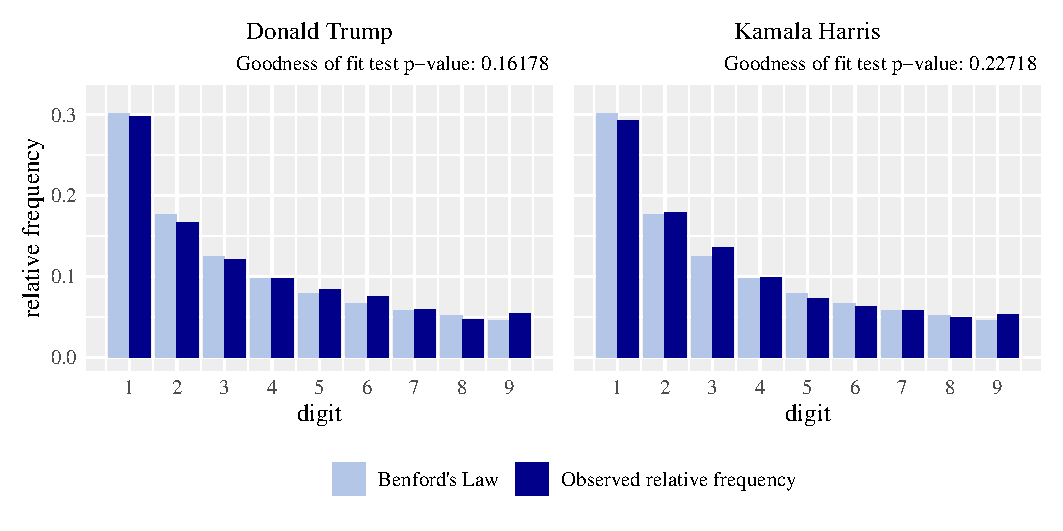
\includegraphics[width=0.99\linewidth]{BT-DT-eng/fig/USA24-dual-first_digits.pdf}
    \label{fig:USA24-dual-first_digits}
\end{figure}

Last digit distribution for both candidates in figure \ref{fig:USA24-dual-last_digits} shows no significant deviations from the BL, and also the null hypothesis is not rejected. 

\begin{figure}[h]
    \centering
    \caption{Last digit distributions from both candidates in the USA in 2024}
    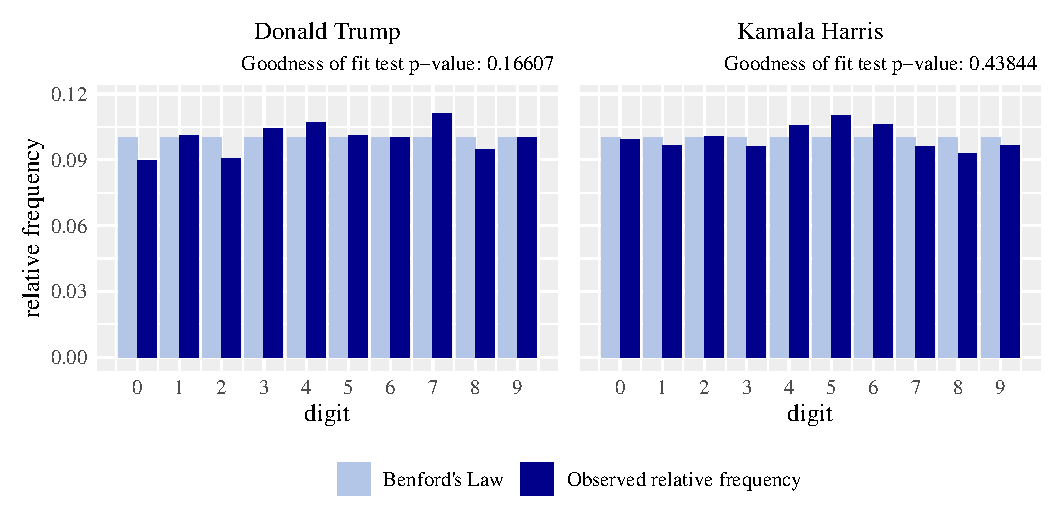
\includegraphics[width=0.99\linewidth]{BT-DT-eng/fig/USA24-dual-last_digits.pdf}
    \label{fig:USA24-dual-last_digits}
\end{figure}

Last but not least, the second leading digits compliance test is not rejected for either of the candidates, as can be seen in figure \ref{fig:USA24-dual-second_digits}. 

\begin{figure}[h]
    \centering
    \caption{Second digit distributions from both candidates in the USA in 2024}
    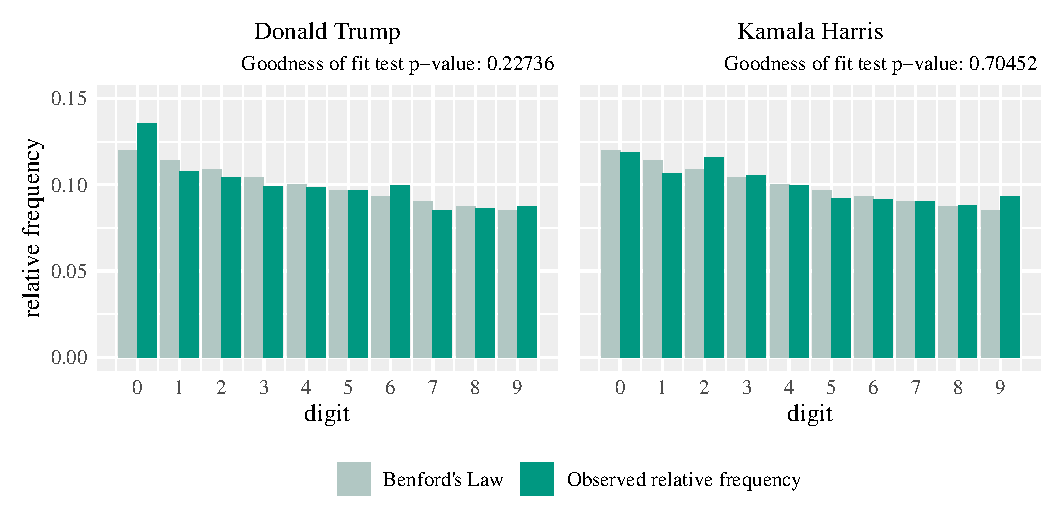
\includegraphics[width=0.99\linewidth]{BT-DT-eng/fig/USA24-dual-second_digits.pdf}
    \label{fig:USA24-dual-second_digits}
\end{figure}

\newpage

\subsubsection{Digital development pattern}

In figure \ref{fig:USA24-digital_development_pattern}, we have observed the development pattern of relative frequencies of the leading digits. In the lower values spectrum, the relative frequencies are not as skewed as we would expect; this is because there is a small fraction of data, so the pattern does not have a chance to develop. In the rest of this bottom quartile, the distribution is closer to equal, with a slight rise towards Benford's first digit law. In the largest partition of the data, the relative frequencies are very close to the law. From there, the first digits are getting much more prevalent. This pattern is in alignment with what \citeauthor{kossovsky2014benford} describes. We have reason to think otherwise. 

\begin{figure}[h]
    \centering
    \caption{Digital development pattern - USA 2024}
    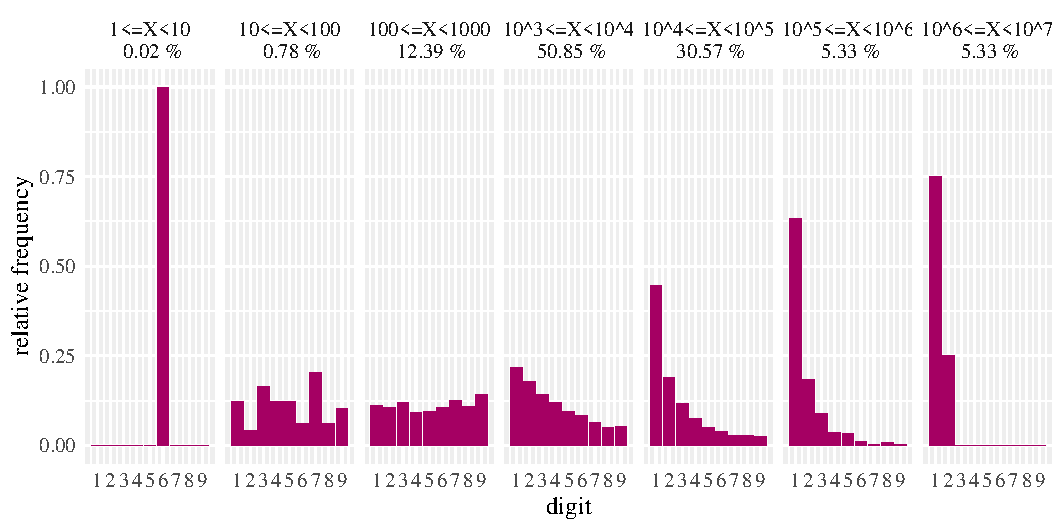
\includegraphics[width=0.99\linewidth]{BT-DT-eng/fig/USA24-digital_development_pattern.pdf}
    \label{fig:USA24-digital_development_pattern}
\end{figure}


% \subsubsection{Results}

% In our tests, we have not acquired enough evidence to suspect fraud of the digital kind.  


%%%%%%%%%%%%%%%%%%%%%%%%%%%%%%%%%%%%

% \section{Russia}
% % https://www.theguardian.com/news/datablog/2012/mar/05/russia-putin-voter-fraud-statistics
% % https://cedarus.io/data/elections

% % https://www.kaggle.com/code/ambarish/benfords-law-and-russian-elections-2018/input?select=voting_data_geo_eng.csv



\newpage 

\section{Presidential elections in Belarus in 2020}

Since the official data was not made public, a sample must suffice for our analysis. This is fine with the BL, since this sample is a fraction of the population, so the law should apply anyway. \citeauthor{BLR20data} are civic youth organisations of the Belarusian opposition. Their members had gathered and processed the final protocols of 1,310 polling stations out of 5,767 throughout Belarus. And these protocols were made available online on Kaggle, this is the data to be analysed in this thesis. \cite{BLR20data}

There were 5 candidates; however, due to their low vote shares, this analysis is focusing mainly on the two most popular candidates - Alexander Lukashenka, former leader and his opponent, Sviatlana Tsikhanouskaya, who took over after her husband was arrested. Lukashenka had ruled for 26 years then, nowadays more than 30. Tsikhanouskaya had been supported by a large fraction of the Belarusian population. The official results speak of 80 \% for Lukashenka and 10 \% for Tsikhanouskaya. Fraud was proven thanks to the Belarusian initiatives Zubr, Honest People and Voice by collecting registered votes from the people, which show that the results should have been very different; their work is visualised by a map, which can be seen in Figure \ref{fig:BLR-fraud-map}. The official election results have not been accepted to this day in the EU, the USA and other democratic societies and have been concluded fraudulent. \cite{Bedford_2021,BLR20data,Voice20}


\begin{figure}[h]
    \centering
    \caption{Presidiential elections in Belarus 2020 - voting places with fraudulent and true results}
    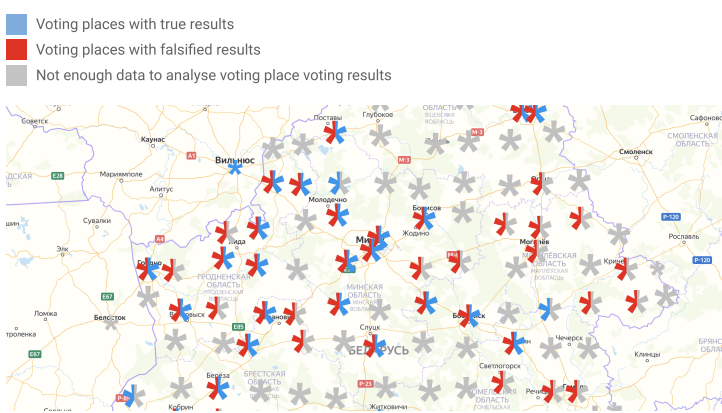
\includegraphics[width=0.75\linewidth]{BT-DT-eng//TemplateBT-DT//img/BLR-fraud-map.png}
    \label{fig:BLR-fraud-map}
    \source{ and processing: \citeauthor{Voice20} in \citeyear{Voice20}}
\end{figure}

These elections were controversial. Demonstrations were happening before and long after the elections. The Belarusian society has awakened in the whole country. Before the elections, some of the candidates were intimidated. The democratic principles of an election were not fulfilled. The OSCE ODIHR were not invited to observe the election and inspect the election integrity. \cite{OBSE-BLR-concern,OBSE-BLR-no-report, Bedford_2021}

\subsubsection{Relative frequencies of the digits on a given position}

Looking at the Figure \ref{fig:BLR20-all-first_digits} showing the first digit distribution and the first digit BL, the plot does not look like much is going on. However, the opposite is true; the goodness of fit test's p-value rejects the null hypothesis that the relative frequencies are equal. For a more detailed view of the first digits distribution, look at the distribution of the first two digits in Figure \ref{fig:BLR20-all-first_two_digits} in the appendix, which also rejected the null hypothesis. 

\begin{figure}[h]
    \centering
    \caption{First digit distribution, Belarus 2020}
    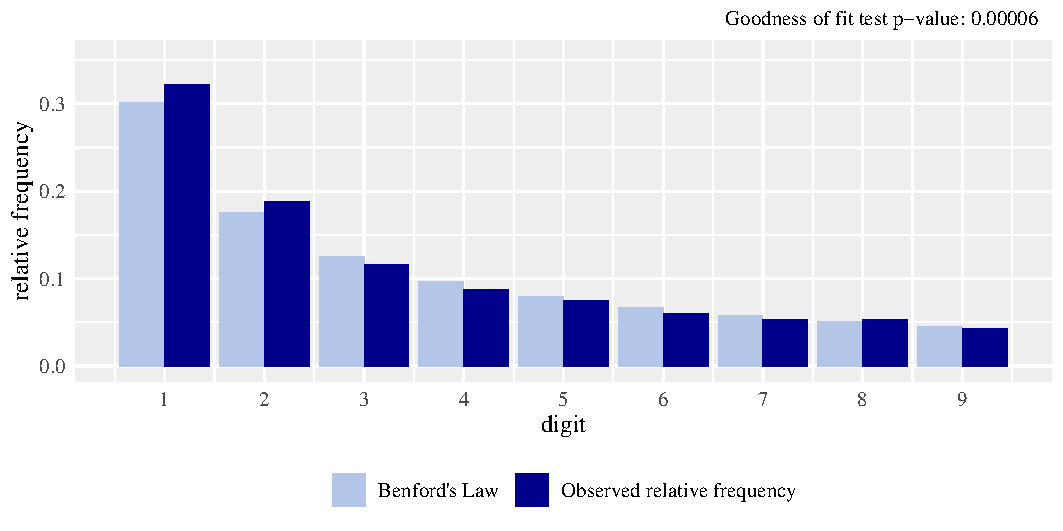
\includegraphics[width=0.99\linewidth]{BT-DT-eng/fig/BLR20-all-first_digits.pdf}
    \label{fig:BLR20-all-first_digits}
\end{figure}

All becomes apparent when the two rivals are plotted separately in Figure \ref{fig:BLR20-dual-first_digits}. For both candidates, the tests provide evidence of fraudulent results. The pattern for Tsikhanouskaya follows the BL more closely than for Lukashenka. His digit distribution is very unusual.

\begin{figure}[h]
    \centering
    \caption{First digit distributions from both candidates in Belarus in 2020}
    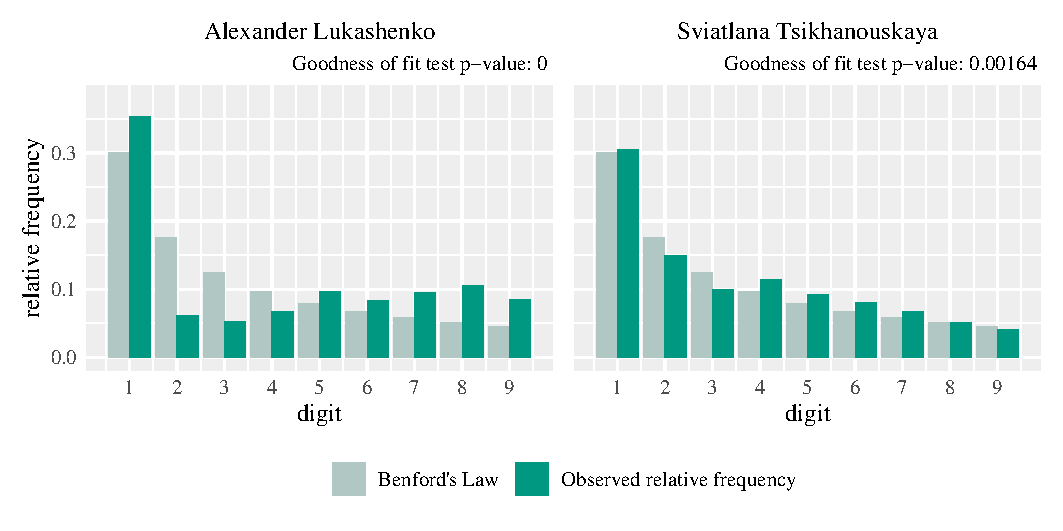
\includegraphics[width=0.99\linewidth]{BT-DT-eng/fig/BLR20-dual-first_digits.pdf}
    \label{fig:BLR20-dual-first_digits}
\end{figure}

Moving on to the next distribution, the last digit distribution in Figure \ref{fig:BLR20-all-last_digits}. The results are much more interesting. For Lukashenko, the results are rejected, for Tsikhanouskaya is not. Reminder that we have set the level of significance to 0.05. This can be interpreted that the results of one candidate were manipulated to a higher degree than the other.  

\begin{figure}[h]
    \centering
    \caption{Last digit distributions from both candidates in Belarus in 2020}
    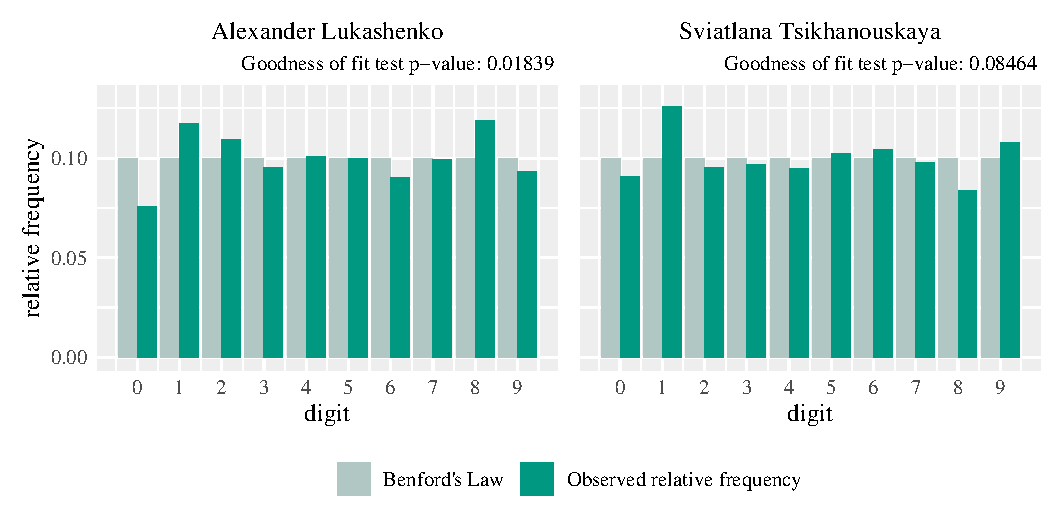
\includegraphics[width=0.99\linewidth]{BT-DT-eng/fig/BLR20-dual-last_digits.pdf}
    \label{fig:BLR20-dual-last_digits}
\end{figure}

And finally, the second digit distribution is quite close to the BL as not disputed by the goodness of fit tests, as can be seen in Figure \ref{fig:BLR20-dual-second_digits}, despite the results from all the vote counts in Figure \ref{fig:BLR20-all-second_digits} rejecting the null. 

\begin{figure}[h]
    \centering
    \caption{Second digit distributions from both candidates in Belarus in 2020}
    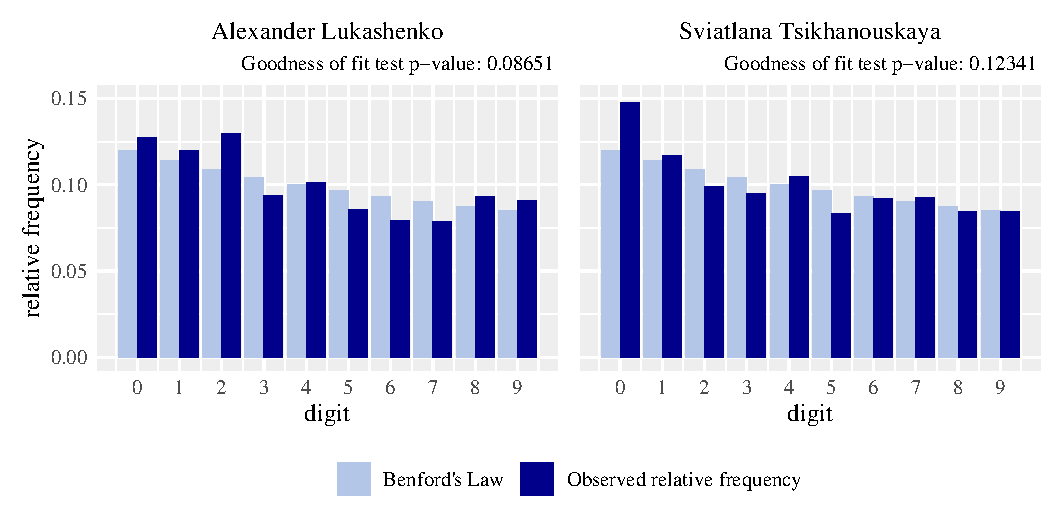
\includegraphics[width=0.99\linewidth]{BT-DT-eng/fig/BLR20-dual-second_digits.pdf}
    \label{fig:BLR20-dual-second_digits}
\end{figure}

Additional plots can be seen in the appendix C, notably the second, third and last digit distributions for all votes in Figures \ref{fig:BLR20-all-third_digits},  \ref{fig:BLR20-dual-third_digits} and \ref{fig:BLR20-all-last_digits}, where for the last digits the null is rejected and for the third digits is not. To see the first two digit distribution for the candidates separately, look at the Figure \ref{fig:BLR20-dual-first_two_digits}. The p-value is unreliable, but the distribution still shows some irregularities. 


\subsubsection{Digital development pattern}

Observing the digital development pattern in Figure \ref{fig:BLR20-digital_development_pattern}, there is not much to see. This is due to the nature of the data itself and the polling stations being similar in size (number of eligible voters in a given region). So there is not much to conclude, however, the tendency is quite similar as to what \citeauthor{kossovsky2014benford} has described. 

\begin{figure}[h]
    \centering
    \caption{Digital development pattern - Belarus 2020}
    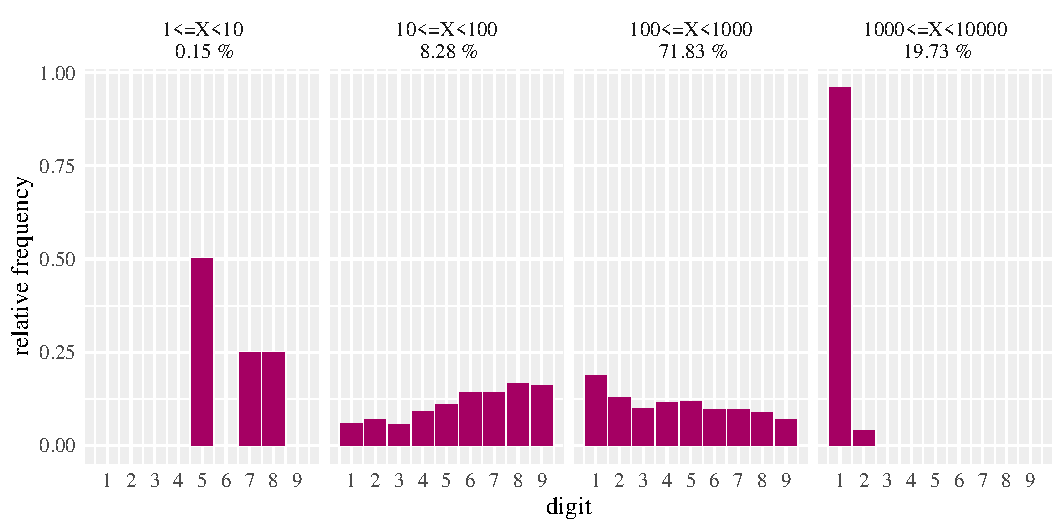
\includegraphics[width=0.99\linewidth]{BT-DT-eng/fig/BLR20-digital_development_pattern.pdf}
    \label{fig:BLR20-digital_development_pattern}
\end{figure}

% \begin{figure}[h]
%     \centering
%     \caption{Scatter}
%     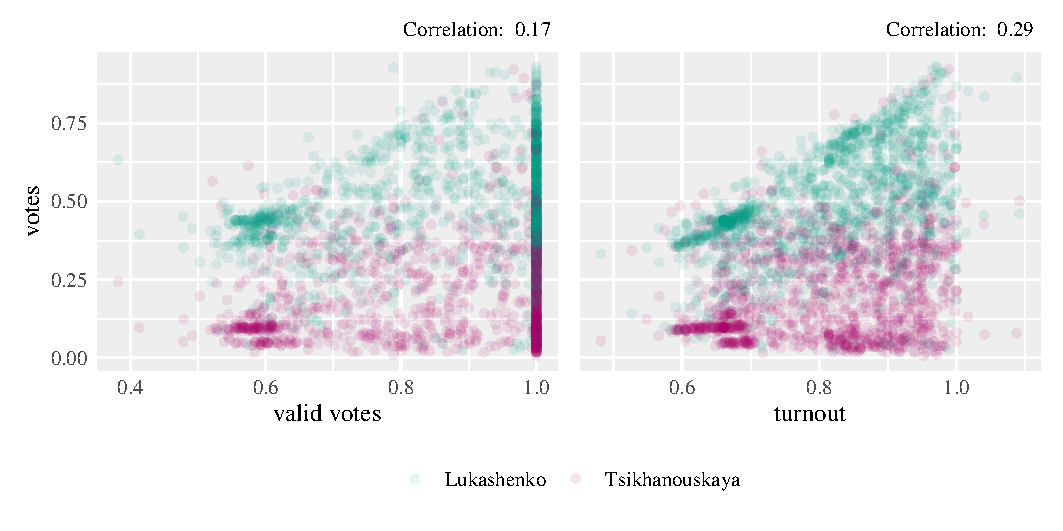
\includegraphics[width=0.99\linewidth]{BT-DT-eng/fig/BLR20-scatter.pdf}
%     \label{fig:BLR20-scatter}
% \end{figure}

% \begin{figure}[h]
%     \centering
%     \caption{Scatter decomposed}
%     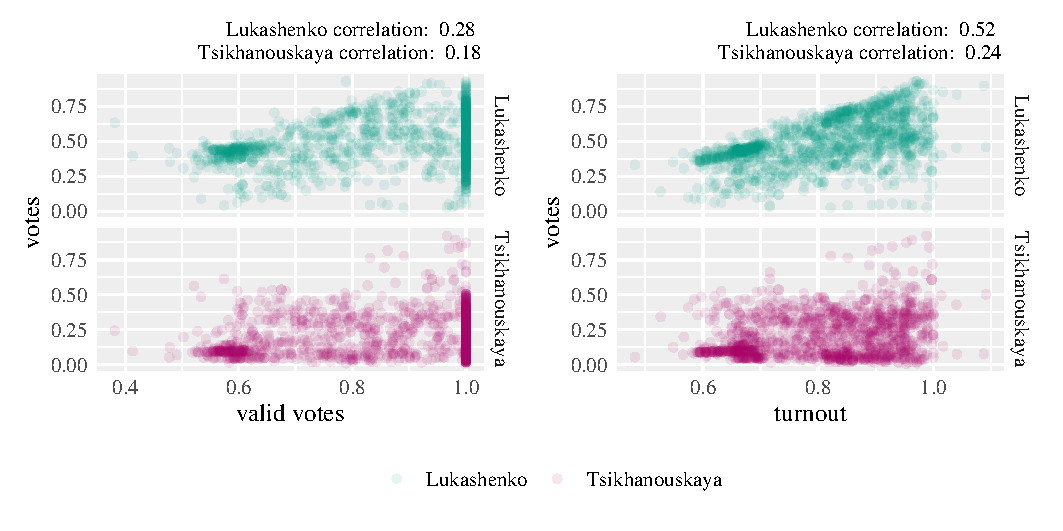
\includegraphics[width=0.99\linewidth]{BT-DT-eng/fig/BLR20-scatter_decompose.pdf}
%     \label{fig:BLR20-scatter-decompose}
% \end{figure}

% \begin{figure}[h]
%     \centering
%     \caption{Digital development pattern}
%     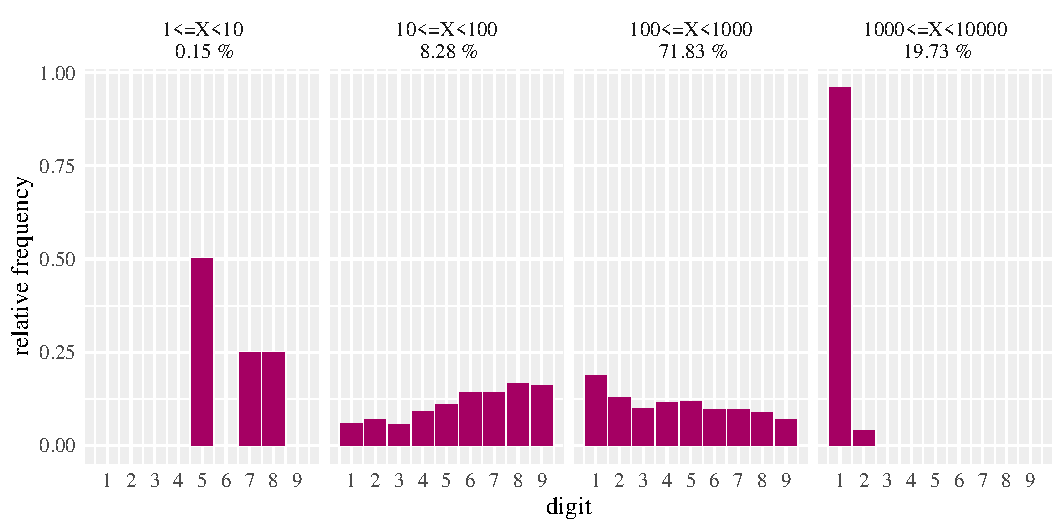
\includegraphics[width=0.99\linewidth]{BT-DT-eng/fig/BLR20-digital_development_pattern.pdf}
%     \label{fig:BLR20-digital_development_pattern}
% \end{figure}

